%!TEX root = ../main.tex
\section{Deep Neural Network Architectures for Locating Anomalies}
\label{sec:locatingAnomalieswithNNArchitecture}


\subsection{Deep Neural Networks}
\label{sec:dnn}
The "deep" in "deep neural networks" refers to the number of layers through which the features of data are extracted~\cite{schmidhuber2015deep,bengio2009learning}. Deep architectures overcome the limitations of traditional machine learning approaches of scalability, and generalization to new variations within data~\cite{lecun2015deep}. Deep Belief Networks (DBNs) are class of deep neural network which comprises of multiple layer of graphical models known as Restricted Boltzmann Machine (RBMs).
The hypothesis in using DBNs for anomaly detection is that RBMs are used as  directed encoder-decoder network that can be trained with backpropogation algorithm~\cite{werbos1990backpropagation}. DBNs fail to learn good representations of anomalous samples, resulting in high reconstruction error. DBNs  are shown to scale efficiently to a large training set and improve interpretability~\cite{wulsin2010semi}.


\subsection{Spatio Temporal Networks (STN)}
\label{sec:stn}
Researchers for long have explored  techniques to learn both both spatial and temporal relation features , since modeling local spatial temporal correlation has wide applications~\cite{zhang2018detecting}. Deep learning architectures have been shown perform well at learning spatial aspects ( using CNNs) and temporal features ( using LSTMs) individually. Spatio Temporal Networks (STNs) comprise of deep neural architectures combining both CNNs and LSTMs to extract spatio-temporal features. The temporal
features (modeling correlations between near time points via LSTM), spatial features (modeling
local spatial correlation via local CNNs) are shown to be effective in detecting outliers~\cite{lee2018stan,szeker2014spatio,nie2018spatio,dereszynski2011spatiotemporal}.

\subsection{ Sum-Product Networks (SPN)}
\label{sec:spn}
Sum-Product Networks (SPNs) are directed acyclic graphs with variables as leaves, while the internal nodes, and weighted edges constitute the sums and products. SPNs are considered as a combination of mixture models ~\cite{poon2011sum,peharz2018probabilistic} which have fast exact probabilistic inference over many layers. The main advantage of SPNs is that, unlike graphical models, SPNs are more traceable over high treewidth models without requiring approximate inference. Furthermore, SPNs are shown to capture uncertainty over their inputs in a convincing manner, yielding robust anomaly detection~\cite{peharz2018probabilistic}. SPNs are shown to be  impressive results on numerous datasets, while much remains to be explored in its application to outlier detection.

\subsection{Word2vec Models}
\label{sec:word2vec}
Word2vec is a group of deep neural network models used to produce word embeddings~\cite{mikolov2013efficient}. These models are capable of capturing sequential relationships within sequential data instance such as sentences, time sequence data. Obtaining word embedding features as inputs is shown to improve the performance in several deep learning architectures~\cite{rezaeinia2017improving,naili2017comparative,altszyler2016comparative}. Word2vec embeddings obtained are also shown to be effective in outlier detection by~\cite{schnabel2015evaluation,bertero2017experience,bakarov2018anomaly,bamler2017dynamic}.


\subsection{Generative Models }
\label{sec:gan_adversarial}

Generative models aim to learn true data distribution in order to generate new data points with some variations. The two most common and efficient generative approaches are Variational Autoencoders (VAE)~\cite{kingma2013auto} and Generative Adversarial Networks (GAN)~\cite{NIPS2014_5423,goodfellow2014generative}. A variant of GAN architecture known as Adversarial autoencoders (AAE) ~\cite{makhzani2015adversarial} that use adversarial training to impose an arbitrary prior on the latent code learnt within hidden layers of autoencoder are also shown to effectively learn the input distribution. Leveraging this ability to learning input distributions several Generative Adversarial Networks-based Anomaly Detection (GAN-AD) techniques ~\cite{li2018anomaly,deecke2018anomaly,schlegl2017unsupervised,ravanbakhsh2017abnormal,eide2018applying}
 proposed are shown to be effective in identifying anomalies in high dimensional and complex datasets  with high detection rate and low false positive rate as compared to state-of-the-art methods. However traditional methods such as K-nearest neighbours (KNN) are shown to perform better in scenarios which have lesser number of anomalies when compared to deep generative models~\cite{vskvara2018generative}.

\subsection{Convolutional Neural Networks }
\label{sec:cnn}
Convolutional Neural Networks (CNNs), are the popular choice of neural networks for analyzing visual imagery~\cite{krizhevsky2012imagenet}. CNNs proved recently to be useful for defining effective data analysis techniques for various applications. CNN’s ability to extract complicated hidden features from high dimensional data with complex structure has enabled its use as feature extractors in outlier detection for both sequential and image dataset~\cite{gorokhov2017convolutional,kim2014convolutional}. Evaluation of CNNs based frameworks for anomaly detection is still an active area of research being explored currently~\cite{kwon2018empirical}.

\subsection{Sequence Models}
\label{sec:rnn_lstm_gru}

Recurrent Neural Networks (RNNs)~\cite{williams1989complexity} are known to capture features of time sequence data. The limitations with RNNs is that they fail to capture the context as time steps increases, in order to resolve this problem,  Long Short-Term Memory~\cite{hochreiter1997long} networks was introduced, they  are a special type of RNNs comprising of memory cell that can store information about previous time steps. Gated Recurrent Unit~\cite{cho2014learning} (GRUs) are similar to LSTMs, but use a set of gates to control the flow of information, instead of separate memory cells. ~\cite{ergen2017unsupervised}
investigate Long Short Term Memory (LSTM) neural network based algorithms for anomaly detection and report significant performance gains achieved over conventional methods. Anomaly detection in sequential data  has attracted significant interest in literature due its applications in a wide range of engineering problems illustrated in Section ~\ref{sec:timeseriesAD}.

\subsection{Autoencoders}
\label{sec:ae}
Autoencoders with single layer alongwith a linear activation function is nearly equivalent to Principal Component Analysis (PCA)~\cite{pearson1901liii}. While PCA is restricted to a linear dimensionality reduction, auto encoders enable both linear or nonlinear tranformations~\cite{liou2008modeling,liou2014autoencoder}. One of the popular applications of Autoencoders is anomaly detection. Autoencoders represent data within multiple hidden layers by reconstructing the input data, effectively learning an identity function. The autoencoders when trained solely on normal data instances ( which are the majority in anomaly detection tasks) fail to reconstruct the anomalous data samples therefore producing a large reconstruction error. The data samples which produce high residual errors are considered outliers. Several variants of autoencoder architectures are proposed as illustrated in Figure ~\ref{fig:aevariants} produce promising results in anomaly detection. The choice of autoencoder architecture depends on the nature of data, convolution networks are preferred for image datasets while Long short-term memory (LSTM) based models tend to produce good results for sequential data. Efforts to combine both convolution and LSTM layers where encoder is a convolutional neural network (CNN) and decoder is a multilayer LSTM network to reconstruct  input images are shown to be effective in both noisy images and sequential data anomaly detection.  The use of combined models  such as Gated Recurrent Unit (GRU-AE), Convolutional Neural Networks Autoencoders (CNN-AE), Long short-term memory (LSTM) autoencoder (LSTM-AE) eliminate the need for preparing hand-crafted features,  and facilitates the use of raw data with minimal preprocessing in anomaly detection tasks.


%%%%% Autoencoder architectures used in anomaly detection %%%%%
\tikzset{edge from parent/.style=
{draw, edge from parent path={(\tikzparentnode.south)
-- +(0,-8pt)
-| (\tikzchildnode)}},
blank/.style={draw=none}}

\begin{figure}
\centering
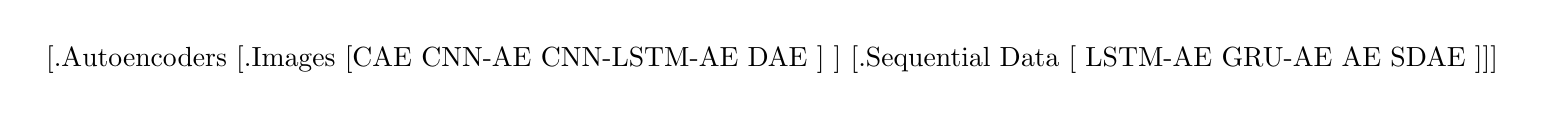
\begin{tikzpicture}
\matrix
{
% \node{\Tree
%     [A.  \edge[blank];
%     [B.  \edge[blank];
%     [C. \edge[blank];
%     [D. ]]]]};
&
\node{\Tree
 [.Autoencoders
    [.Images
        [{CAE} {CNN-AE}  {CNN-LSTM-AE} {DAE} ] ]
    [.{Sequential Data}
            [ {LSTM-AE} GRU-AE AE SDAE ]]]};\\
};
\end{tikzpicture}
\caption{\textbf{Autoencoder architectures for anomaly detection}.
        \\AE: Autoencoders~\cite{liou2014autoencoder}, LSTM : Long Short Term Memory Networks~\cite{hochreiter1997long}
        \\SDAE: Stacked Denoising Autoencoder~\cite{vincent2010stacked}, DAE : Denoising Autoencoders~\cite{vincent2010stacked}
        \\GRU: Gated Recurrent Unit~\cite{cho2014learning}, CNN: Convolutional Neural Networks~\cite{krizhevsky2012imagenet}
        \\CNN-LSTM-AE: Convolution Long Short Term Memory Autoencoders~\cite{haque2018image}
        \\CAE: Convolutional Autoencoders~\cite{masci2011stacked}
        }

 \label{fig:aevariants}
\end{figure}
Autoencoders are simple and effective architectures for outlier detection. However, the performance gets degraded  due to noisy training data with a large fraction of corruptions~\cite{zhou2017anomaly}.

